\input{BeamerSettings}

\definecolor{codegreen}{rgb}{0,0.6,0}
\definecolor{codegray}{rgb}{0.5,0.5,0.5}
\definecolor{codepurple}{rgb}{0.58,0,0.82}
\definecolor{backcolour}{rgb}{0.95,0.95,0.92}

\lstdefinestyle{mystyle}{
    backgroundcolor=\color{backcolour},   
    commentstyle=\color{codegreen},
    keywordstyle=\color{magenta},
    numberstyle=\tiny\color{codegray},
    stringstyle=\color{codepurple},
    basicstyle=\ttfamily\tiny,
    breakatwhitespace=false,         
    breaklines=true,                 
    captionpos=b,                    
    keepspaces=true,                 
    numbers=left,                    
    numbersep=5pt,                  
    showspaces=false,                
    showstringspaces=false,
    showtabs=false,                  
    tabsize=2,
    xleftmargin=0.05\textwidth,
    xrightmargin=0.45\textwidth	
}

\AtBeginSection[]{
  \begin{frame}[noframenumbering]
  \vfill
  \centering
  \begin{block}{}
    \usebeamerfont{title}\insertsectionhead\par
  \end{block}
  \vfill
  \end{frame}
}

\newcommand{\inlinecode}[1]{\colorbox{backcolour}{\lstinline{#1}}}

\lstset{style=mystyle}

\author[RMR]{\textbf{Ryan~M.~Richard}}
\title[Git \& GitHub]{Version Control, Git, and GitHub}
\institute[Ames]{
	Scientist and Adjunct Assistant Professor of Chemistry\\
	Ames National Laboratory and Iowa State University\\
	Ames, IA, USA
} 

\date[6-4-2026]{2026 SIMCODES Bootcamp}

\begin{document}
\TitleSlide

\section{Why Do We Need Version Control?}

\TwoColumnSlide{Motivation}
{\BulletList{
\item Imagine three people are trying to write this presentation.
\item Assume their parents named them A, B, and C.
\item Also assume these people haven’t heard of Google Slides or Office 365 and are trying to do this via email.
\item Assume the slides are supposed to be ordered so that A’s slides come first, B’s come second, and C’s third.
\item Let’s work through some scenarios in gether.
}}
{
\AddPicture{motivation.png}
}
{}

\TwoColumnSlide{Scenario 1: Linear History (i.e., the history no time travel movie has)}
{\BulletList{
\item A makes their slides and emails the presentation to B. 
\item B adds their slides to the presentation A sends.
\item B emails  the presentation to C. 
\item C adds their slides.
\item Presentation is done. 
\item Called a “linear history” because the timeline has no “branches.”
\begin{itemize}
\item “Branches” are easier to define when we have one. 
\end{itemize}
}}
{\AddPicture{scenario1.png}}
{}

\TwoColumnSlide{Scenario 2: Non-conflicting branched history (i.e., the timeline every time travel movie thinks it has)}
{\BulletList{
\item A makes their slides.
\item  A sends the slides to both B and C.
\item Simultaneously:
\begin{itemize}
	\item B adds slides in the correct place.
	\item C adds slides in the correct place.
\end{itemize}
\item The two presentations are ``magically'' merged.
\item “Branched history” because different changes happen simultaneously.
}}
{\AddPicture{scenario2.png}}
{}

\TwoColumnSlide{Scenario 3: The conflicting branched timeline (i.e., the timeline every time travel movie actually has)}
{\BulletList{
\item A makes their slides.
\item Slides sent to both B and C.
\item Simultaneously:
\begin{itemize}
	\item B appends their slides.
	\item C appends their slides.
\end{itemize}
\item Conflict: both B and C think their slides come directly after A.
\item ``Magic'' merging moves C’s slides to the end.
\item “Branched history” because different changes happen simultaneously.
\item “Conflicting” because the histories are not compatible.
}}
{\AddPicture{scenario3.png}}
{}

\TwoColumnSlide{Motivation Summary}
{\BulletList{
\item Having multiple people work on the same file can be difficult without coordination.
\item Guess what happens when we have multiple people work on multiple files without coordination?
\item Modern software development almost always involves multiple people working on multiple files in an uncoordinated (or loosely coordinated) manner.
}}
{\AddPicture{avengers_timeline.jpg}}
{}

\section{What is the Difference Among Version Control, Git, and GitHub?}

\TwoColumnSlide{What is Version Control (VC)?}
{\BulletList{
\item VC software is used to manage the history (i.e., versions) of a software project.
\item Superficially, VC gives you save/load, undo, redo for a set of files.
\item Automates (to the extent possible) the steps we termed “magic.”
\item Historically, there have been many different VC software packages.
\item Now, most developers (95\% according to Wikipedia) have coalesced around Git.
}}
{\AddPicture{what_is_vc.jpg}}
{}

\TwoColumnSlide{What is Git?}
{\BulletList{
\item Developed by Linus Torvalds for version controlling the Linux kernel.
\begin{itemize}
	\item Written because a proprietary VC software company revoked Linux community's free license.
	\item Amusingly outperformed all other existing VC software after three weeks of development.
\end{itemize}
\item According to Linus, git's meaning depends on your mood:
\begin{itemize}
	\item “Global information tracker” if you’re in a good mood.
	\item “Goddamn idiotic truckload of sh*t” when it breaks.
\end{itemize}
}}
{\AddPicture{what_is_git.png}}
{}

\TwoColumnSlide{What is GitHub?}
{\BulletList{
\item For SIMCODES we are using Git in the context of GitHub.
\item Git is the software responsible for VC-ing our software project.
\item GitHub is “just” a storage solution (e.g., like Google Drive or DropBox).
\item Use Git to interact with GitHub.
}}
{\AddPicture{github.jpg}}
{}

\section{Git and GitHub Terminology}

\TwoColumnSlide{Disclaimer: Simplifications Ahead}
{\BulletList{
\item Git is a powerful VC solution.
\item Power comes from not assuming any “sacred timeline.”
\item Leads to additional levels of abstraction that complicate things. 
\item Simplified by noting that the copy on GitHub is treated specially.
\item The git Jedis in the room know that there’s exceptions to pretty much everything I’m about to tell you.
}}
{\AddPicture{disclaimer.jpg}}
{}

\TwoColumnSlide{Term: Repository}
{\BulletList{
\item A \textbf{repository} contains the source files and the history of changes to those files.
\item A \textbf{local} repository is a repository that lives on the computer you are currently using.
\begin{itemize}
	\item You always develop software in a local repository.
\end{itemize}
\item A \textbf{remote} repository is a repository that lives on a different computer.
\begin{itemize}
	\item Assume  ”remote” is synonymous with “the repository that lives on GitHub”.
\end{itemize}
\item Repository is usually shortened to just “repo.”
}}
{\AddPicture{folder.png}}
{}

\TwoColumnSlide{Term: Clone}
{\BulletList{
\item The first step in developing software is to get a copy of the existing source code.
\item Usually, the repo you want to develop for already lives on GitHub.
\item To get a local copy of a remote repo you \textbf{clone} it.
\item Unless you delete your local repo, you typically only clone a repo once.
}}
{\AddPicture{clone.jpg}}
{}

\TwoColumnSlide{Term: Branch}
{\BulletList{
\item A \textbf{branch} is a (linear) history of the repo.
\begin{itemize}
	\item It’s one of the many timelines.
\end{itemize}
\item Usually, one branch is special.
\begin{itemize}
	\item Often called the \textbf{main} or \textbf{master} branch.
\end{itemize}
\item The special branch is the ”final” version of the project.
\item Other branches are sometimes called development branches.
\item You should ALWAYS be working on a development branch.
}}
{\AddPicture{branch.png}}
{}

\TwoColumnSlide{Term: Commit}
{\BulletList{
\item Git doesn’t come with “auto-save”.
\item A \textbf{commit} is the set of changes you made to the branch since the last commit.
\begin{itemize}
	\item Conceptually, a commit is Git’s equivalent of “saving”.
	\item In the timeline analogy, commits are events.
\end{itemize}
\item Commits can add content and/or remove content.
\item Commits save your work on the current branch. Other branches remain unchanged.
}}
{\AddPicture{commit.png}}
{}

\TwoColumnSlide{Terms: Push, Pull, Merge}
{\BulletList{
\item When you are done developing a feature locally you need to add the feature to the remote repo.
\item You \textbf{push} your changes from your local branch to the remote branch.
\item You \textbf{pull} changes from a remote branch to your local branch.
\item If you are moving changes from one local branch to another local branch you \textbf{merge} the branches. 
\item As a note, pushing and pulling are implemented in terms of merge, so “merge” is usually used as a catchall.
}}
{\AddPicture{pull.jpg}}
{}

\TwoColumnSlide{Term: Conflict}
{\BulletList{
\item Git is pretty good about merging changes automatically.
\item However, when the same lines of code have been modified, Git usually needs help merging.
\item When Git cannot automatically merge two branches, the branches are said to be in conflict.
\item If a conflict occurs Git will show you the two changes and you will have to decide how to reconcile them.
}}
{\AddPicture{conflict.jpg}}
{}

\TwoColumnSlide{Term: Organization}
{\BulletList{
\item Developer teams usually work on a series of related projects.
\begin{itemize}
	\item E.g., the SIMCODES team has one project for the website, one project for training materials, and several projects for research.
\end{itemize}
\item Git provides no mechanism for grouping repositories (we don’t speak of git submodule…).
\item A GitHub \textbf{organization} allows a developer team to group their repos together.
\item SIMCODES has the GitHub organization SIMCODES-ISU (SIMCODES was taken…). 
}}
{}
{}

\TwoColumnSlide{Term: Pull Request}
{\BulletList{
\item A \textbf{pull request} (or PR for short) tells the maintainers of a GitHub repo that you want them to pull changes into their repo.
\begin{itemize}
	\item The repo owners can then decide if they want those changes or not.
\end{itemize}
\item PRs are needed because we don'tt want just anyone making changes to our code.
\item Most repos now require PRs, regardless of who is making changes.
\begin{itemize}
	\item PRs are used to automatically test changes before merging them.
\end{itemize}
}}
{\AddPicture{pull_request.jpg}}
{}

\TwoColumnSlide{Term: Fork}
{\BulletList{
\item PRs must be between branches that live on GitHub.
\item If you have sufficient privileges, then create a branch and make a PR. 
\begin{itemize}
	\item But what if you don’t have sufficient privileges?
\end{itemize}
\item A GitHub \textbf{fork} is a clone of a GitHub repository that you own.
\begin{itemize}
	\item Can make the PR from a branch of your fork.
\end{itemize}
\item Even if you have permission to create a branch in a repo, you can always fork the repo and make a PR from the fork.
}}
{\AddPicture{fork.png}}
{}

\section{Git/GitHub Workflow}

\TwoColumnSlide{Public Service Announcement}
{\BulletList{
\item If you follow these steps, every single time you develop software you will rarely (if ever) encounter a Git/GitHub problem.
\begin{itemize}
	\item Disclaimer: problem is not the same as “conflict”, though this workflow will greatly reduce conflicts too!
\end{itemize}
\item If you don’t follow these steps, you can still accomplish your goals, but you will make life 10x harder for yourself.
\item In my experience, 99\% of Git problems come from skipping one of theses steps.
}}
{\AddPicture{psa.jpg}}
{}

\TwoColumnSlide{Hands-on Example}
{\BulletList{
\item We will make a small change to the README.md file.
\item Look at the README.md file and identify a way to improve it.
\begin{itemize}
	\item Add the NSF acknowledgement.
\end{itemize}
}}
{\AddPicture{readme.png}}
{}

\TwoColumnSlide{Step 1: Make a Feature Branch}
{\BulletList{
\item<1->You should NEVER make changes to the main/master branch!
\begin{itemize}
	\item<1-> Exception: None. There is no exception!
	\item<1-> But what about if…No! Don’t do it!
\end{itemize}
\item <1-> In my experience, making changes directly to the main/master branch is the primary way Git newbies get in a pickle.
\item<2-> You start on the ``main'' branch.
\item<3-> Click on branch name to manage branches.
}}
{
\only<1>{\AddPicture<1>{main_branch.png}}
\only<2>{
\begin{center}
\includegraphics<2>[scale=0.12,keepaspectratio]{main_branch.jpg}
\end{center}
}
\only<3>{\AddPicture<3>{create_new_branch.jpg}}
\only<4>{\AddPicture<4>{branch_name.jpg}}
\only<5>{\AddPicture<5>{branch_name_changed.jpg}}
}
{}

\TwoColumnSlide{Step 2: Make Some Changes}
{\BulletList{
\item Here we added the NSF acknowledgement.
\item Make the changes you identified earlier.
\item Ensure you save the file.
}}
{\AddPicture{make_changes.jpg}}
{}

  \TwoColumnSlide{Check Your Understanding}
  {
  \vfill
  \centering
  \begin{block}<1-2>{How do we save the changes using git?}
  \only<2>{By committing them.}
  \end{block}
  \vfill
  }
  {\only<2>{\AddPicture{commit_funny.jpg}}}
{}

\TwoColumnSlide{Step 3: Commit the Changes}
{\BulletList{
\item<1-> Switch to the VC view to see the status of all repos in your workspace.
\item<2-> Write a meaningful commit message.
\item<3-> Stage the changes you want to commit.
\item<4-> Click ``Commit''.
}}
{

\only<1>{\AddPicture{git_view.jpg}}
\only<2>{\AddPicture{commit_message.jpg}}
\only<3>{\AddPicture{staged.jpg}}
\only<4>{\AddPicture{committed.jpg}}
}
{}

\TwoColumnSlide{Aside: First commit}
{\BulletList{
\item<1-> If this is the very first time you have made a commit you will get an error message.
\item<2-> Set the email and username.
}}
{
\only<1>{\AddPicture{first_git_use.jpg}}
\only<2>{\AddPicture{git_settings.jpg}}
}
{}

\TwoColumnSlide{Step 4: Push the Changes}
{\BulletList{
\item<1-> Now the changes are saved locally, but not remotely.
\item<2-> Click ``Publish Branch'' (first time pushing this branch) or ``Synch Changes'' (subsequent pushes).
\item<3->  VSCode needs permissions to push to GitHub.
\item<4-> Will take you to your browser so you can sign in.
}}
{
\only<1>{\AddPicture{git_push_funny.png}}
\only<2>{\AddPicture{committed.jpg}}
\only<3>{\AddPicture{signin_to_github.jpg}}
\only<4>{\AddPicture{github_signin.jpg}}
}
{}

\TwoColumnSlide{Step 5: Make a PR}
{\BulletList{
\item <1-> Your GitHub repo should display a “Compare \& pull request” button. Click it.
\item <2-> You now need to fill out the next page.
\begin{itemize}
	\item<2-> Tell people what you did (and plan to do).
	\item<2-> Pick who will review your PR (pick your mentor)
	\item<2-> Assignees are working on the PR (click ”assign yourself”).
	\item<2-> Ignore the rest, click “Create pull request”.
\end{itemize}
\item<2-> Only done once per branch.
\item<2-> If you have more changes, go back to step 2.
}}
{
\only<1>{\AddPicture{compare_and_pr.png}}
\only<2>{\AddPicture{make_pr.png}}
}
{}

\TwoColumnSlide{Step 6: Code Review}
{\BulletList{
\item Maintainers of the remote repo decide if your changes can/should be merged or not.
\item Code review usually involves automated and human checks.
\begin{itemize}
	\item Automated checks run your changes and see if they work.
	\item Reviewers will also look over your changes and may request changes.
\end{itemize}
\item If you pass code review, the maintainers will merge your PR.
\item If you do not pass code review, you go back to Step 2 to make the requested changes.
}}
{\AddPicture{code_review.png}}
{}

  \begin{frame}[noframenumbering]
  \vfill
  \centering
  \begin{block}<1-2>{What does merging a PR accomplish?}
  \only<2>{Adds your changes to the main branch}
  \end{block}
  \vfill
  \end{frame}

\TwoColumnSlide{Step 7: Resetting}
{\BulletList{
\item<1-> Do NOT continue to keep making changes to a merged branch!
\item<1-> We need to ``reset'' so we are again ready for step 1.
\begin{itemize}
	\item<2-> Switch to ``main'' (like Step 1, but pick ``main'' not create new branch).
	\item<2-> In git view, click ``Sync Changes''
\end{itemize}
\item<2-> Skipping this step will cause histories to diverge.
}}
{
\only<1>{\AddPicture{resetting.jpg}}
\only<2>{\AddPicture{synch_main.png}}
}
{}

\TwoColumnSlide{Summary}
{\BulletList{
\item We strongly recommend following this workflow every time you make changes!
\item With practice, steps 1- 4 take seconds.
\item This workflow easily scales to development of multiple features.
\begin{itemize}
	\item Stick with a single feature when you first start out.
\end{itemize}
\item NEVER skip steps 1 and 7!!!
}}
{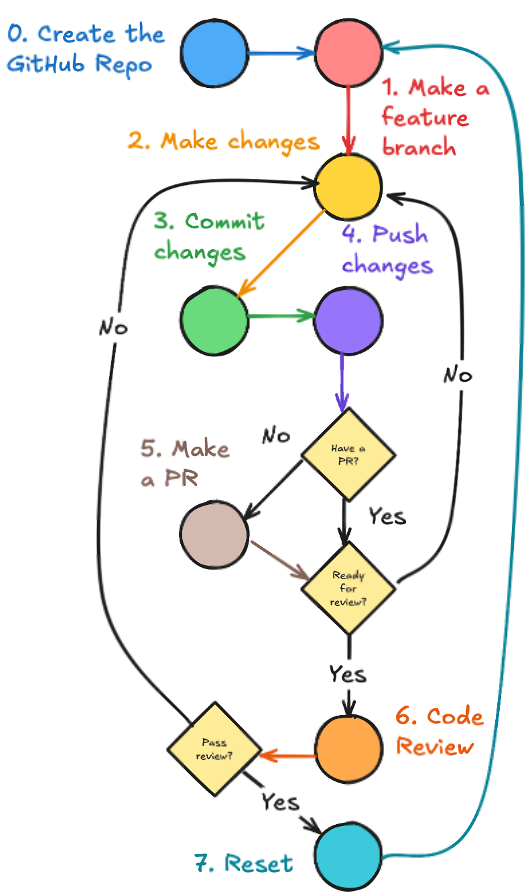
\includegraphics[scale=0.5,keepaspectratio]{summary.png}}
{}

\TwoColumnSlide{Take Aways}
{\BulletList{
\item Collaborating on multiple files with multiple people is difficult.
\item Version control (VC) makes the process much less painful.
\begin{itemize}
	\item We use Git for VC and GitHub for storing our repos.
\end{itemize}
\item Software development follows the same workflow every time.
\item Deviating from the workflow will increase the likelihood of conflicts, or other problems, arising from when you try to pull or push.
}}
{\AddPicture{bad_time.jpg}}
{}

\TwoColumnSlide{Acknowledgements}
{\BulletList{
	\item MolSSI’s git tutorials.
	\item MolSSI’s GitHub tutorials.
	\item NSF for funding the REU.
	\item ISU and Ames National Lab
}}
{
	\AddPicture{molssi.png}
	\AddPicture{nsf.jpg}
}
{}

\end{document}
